
\subsection{Presentation Layer}
Præsentationslaget i kasseapparatet er opbygget med XML i WPF. Selve laget blev først designet ved brug af skitsen på figur \ref{fig:KasseMockup} og derefter implementeret i visual studios WPF designer som set på figur \ref{fig:EndeligeGUI}. Da Grænsefladen var sat op så blev yderligere underliggende funktionalitet tilføjet såsom viewmodels. Disse vil blive forklaret i næste afsnit.

\begin{figure}[H]
	\centering
	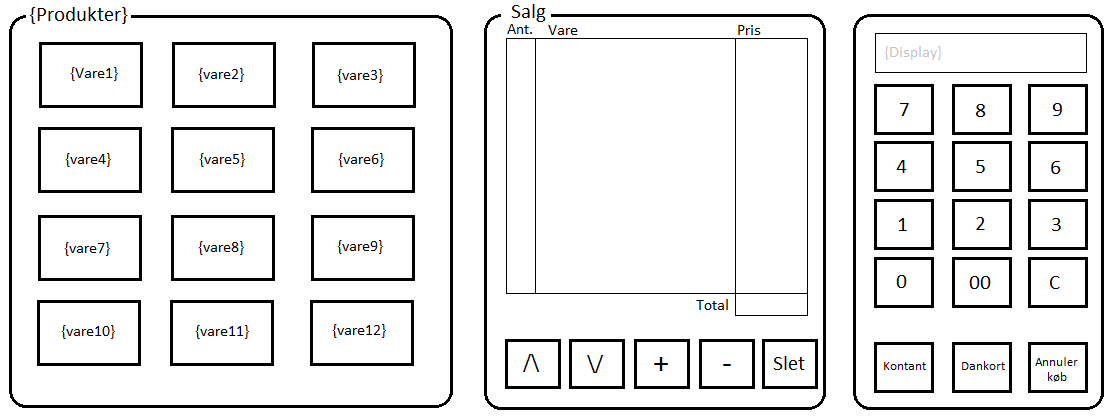
\includegraphics[width=1\textwidth]{Systemdesign/Frontend/pics/KasseMockup}
	\caption{Første mockup af grænsefladen til kasseapparatet.}
	\label{fig:KasseMockup}
\end{figure}

Denne skitse implementerede vi så.

\begin{figure}[H]
	\centering
	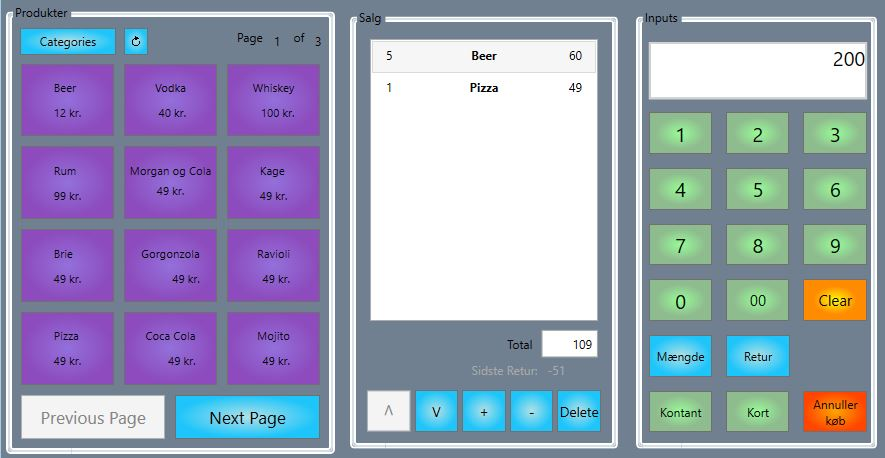
\includegraphics[width=1\textwidth]{Systemdesign/Frontend/pics/GUI}
	\caption{ProductButtonControl}
	\label{fig:EndeligeGUI}
\end{figure}

Da grænsefladen var opsat var det nu nødvendigt at opsætte viewmodels til at forbinde grænsefladen med de underliggende lag.

\subsubsection{ViewModels}

\subsubsection{Klassebeskrivelser}
\textbf{CategoriesMenu}


\textbf{MenuCategory}

\textbf{ProductButtonControl} \\
ProductButtonControl står for at styre hvilken knappeside der vises. Dette betyder at den indeholder en ProduktButtonList, der ved klik er i stand til at skifte knappeside.

\begin{figure}[H]
	\centering
	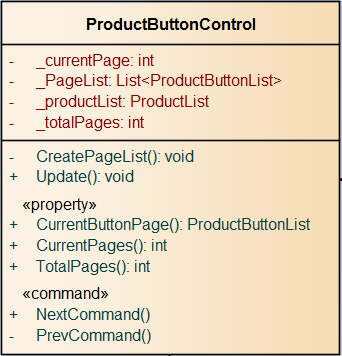
\includegraphics[width=0.3\textwidth]{Systemdesign/Frontend/pics/ProductButtonControl}
	\caption{ProductButtonControl.}
	\label{fig:PBC}
\end{figure}

\textbf{ProductButtonList} \\
ProductButtonList indeholder lister af knapper. Derved kan hver knappeliste symbolisere en side af knapper. Denne liste har ikke nogen anden funktionalitet, men eksisterer for at koden skal kunne facilitere dynamiske knappestørrelser i fremtiden. Denne klasse ville kunne tjekke på hvor stor siden er, og oprette knappesider med den ønskede antal knapper derefter.


\begin{figure}[H]
	\centering
	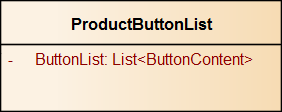
\includegraphics[width=0.3\textwidth]{Systemdesign/Frontend/pics/ProductButtonList}
	\caption{ProductButtonList.}
	\label{fig:PBL}
\end{figure}

\textbf{ProductButtonContent} \\
ProductButtonContent har indholdet af 1 knap på grænsefladen, samt produktinformationer og commands til at oprette produkter på shoppinglist ved tryk. Når man skifter side i grænsefladen produktbuttoncontent være forbundet til hver knap.

\begin{figure}[H]
	\centering
	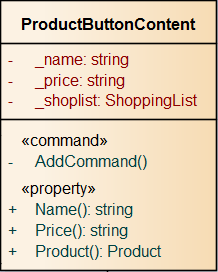
\includegraphics[width=0.2\textwidth]{Systemdesign/Frontend/pics/ProductButtonContent}
	\caption{ProductButtonContent.}
	\label{fig:PBCon}
\end{figure}




